\documentclass[conference]{IEEEtran}
\usepackage{amsmath,amssymb}
\usepackage{booktabs}
\usepackage{graphicx}
\usepackage{cite}
\usepackage{tikz}

\begin{document}

% Put your paper title here. Keep it under about 15 words.
\title{Low-Latency Scheduling for Edge Inference on Shared Accelerators}

% One \IEEEauthorblockN / \IEEEauthorblockA pair per author.
\author{
\IEEEauthorblockN{First Author}
\IEEEauthorblockA{Dept. of Computer Engineering\\Example University\\City, Country\\first.author@example.edu}
\and
\IEEEauthorblockN{Second Author}
\IEEEauthorblockA{Systems Lab\\Sample Institute\\City, Country\\second.author@example.org}
}

\maketitle

\begin{abstract}
Summarise the problem, your approach and the headline result in roughly 150 words.
Conference reviewers often read only this paragraph, so make every sentence count.
\end{abstract}

\begin{IEEEkeywords}
edge computing, scheduling, deep learning inference, accelerators
\end{IEEEkeywords}

\section{Introduction}
Motivate the problem and list your contributions. A short bulleted list works well:
\begin{itemize}
  \item a new scheduling policy that bounds tail latency;
  \item an open implementation on commodity hardware;
  \item an evaluation on three public workloads.
\end{itemize}

\section{Related Work}
Group earlier approaches by idea rather than by paper \cite{smith2020,chen2022}.

\section{System Design}
Describe the architecture. Fig.~\ref{fig:arch} shows where a diagram would go.

\begin{figure}[t]
  \centering
  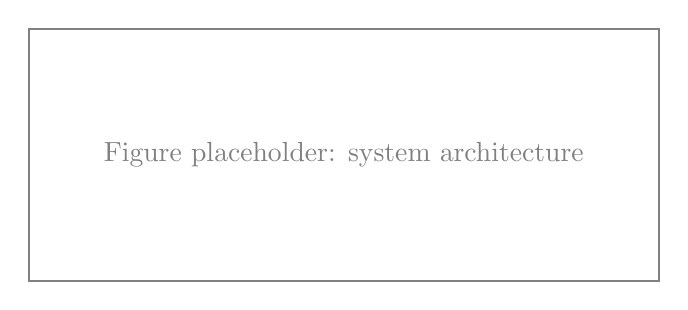
\begin{tikzpicture}
    \draw[thick,gray] (0,0) rectangle (8,3.2);
    \node[gray] at (4,1.6) {Figure placeholder: system architecture};
  \end{tikzpicture}
  \caption{Overview of the proposed scheduler.}
  \label{fig:arch}
\end{figure}

The queueing delay for request $i$ is modelled as
\begin{equation}
  d_i = w_i + \frac{s_i}{\mu - \lambda},
\end{equation}
where $\lambda$ is the arrival rate and $\mu$ the service rate.

\section{Evaluation}
Explain the setup, then present results as in Table~\ref{tab:results}.

\begin{table}[t]
  \centering
  \caption{Tail latency in milliseconds (placeholder values)}
  \label{tab:results}
  \begin{tabular}{lccc}
    \toprule
    Method & p50 & p95 & p99 \\
    \midrule
    FIFO baseline & 12.4 & 48.1 & 97.3 \\
    Priority queue & 11.9 & 35.6 & 70.2 \\
    \textbf{Ours} & \textbf{11.2} & \textbf{22.8} & \textbf{31.5} \\
    \bottomrule
  \end{tabular}
\end{table}

\section{Conclusion}
Restate the contribution and name one direction for future work.

\section*{Acknowledgment}
Funding sources go here. Note the American spelling used by IEEE.

\begin{thebibliography}{1}
\bibitem{smith2020} A.~Smith and B.~Jones, ``Batching strategies for neural inference,'' in \emph{Proc. Example Conf. Systems}, 2020, pp.~101--110.
\bibitem{chen2022} L.~Chen, ``Accelerator sharing in multi-tenant clusters,'' \emph{Example Trans. Computers}, vol.~71, no.~4, pp.~880--893, 2022.
\end{thebibliography}

\end{document}
